\documentclass{mypaper}

\title{Manual til \texttt{svg2ais} og \texttt{plotais}}
\author{Kristian Kjærgaard}
\date{\today}

\usepackage{tikz}

\begin{document}

\maketitle

Her skal der stå en forklaring til fremgangsmåden i programmet. De
ting, jeg ikke selv er helt med på, skal fremgå her.

Ting, der skal dokumenteres:

\begin{itemize}
\item Afstandsfunktionen i Line dst underscore line
\item Algoritmen til at optimere afstanden skal pædagogiseres
\end{itemize}

Sådan gør jeg: Indlæs figuren. Hvert element er en ``Shape''.

\begin{figure}[htbp]
  \centering
  % Graphic for TeX using PGF
% Title: /home/kristian/Dokumenter/HTX/El/Projekter/Eksamensprojekt/svn/trunk/svg2ais/doc/obj-oversigt.dia
% Creator: Dia v0.96.1
% CreationDate: Sat Jan  3 18:47:19 2009
% For: kristian
% \usepackage{tikz}
% The following commands are not supported in PSTricks at present
% We define them conditionally, so when they are implemented,
% this pgf file will use them.
\ifx\du\undefined
  \newlength{\du}
\fi
\setlength{\du}{15\unitlength}
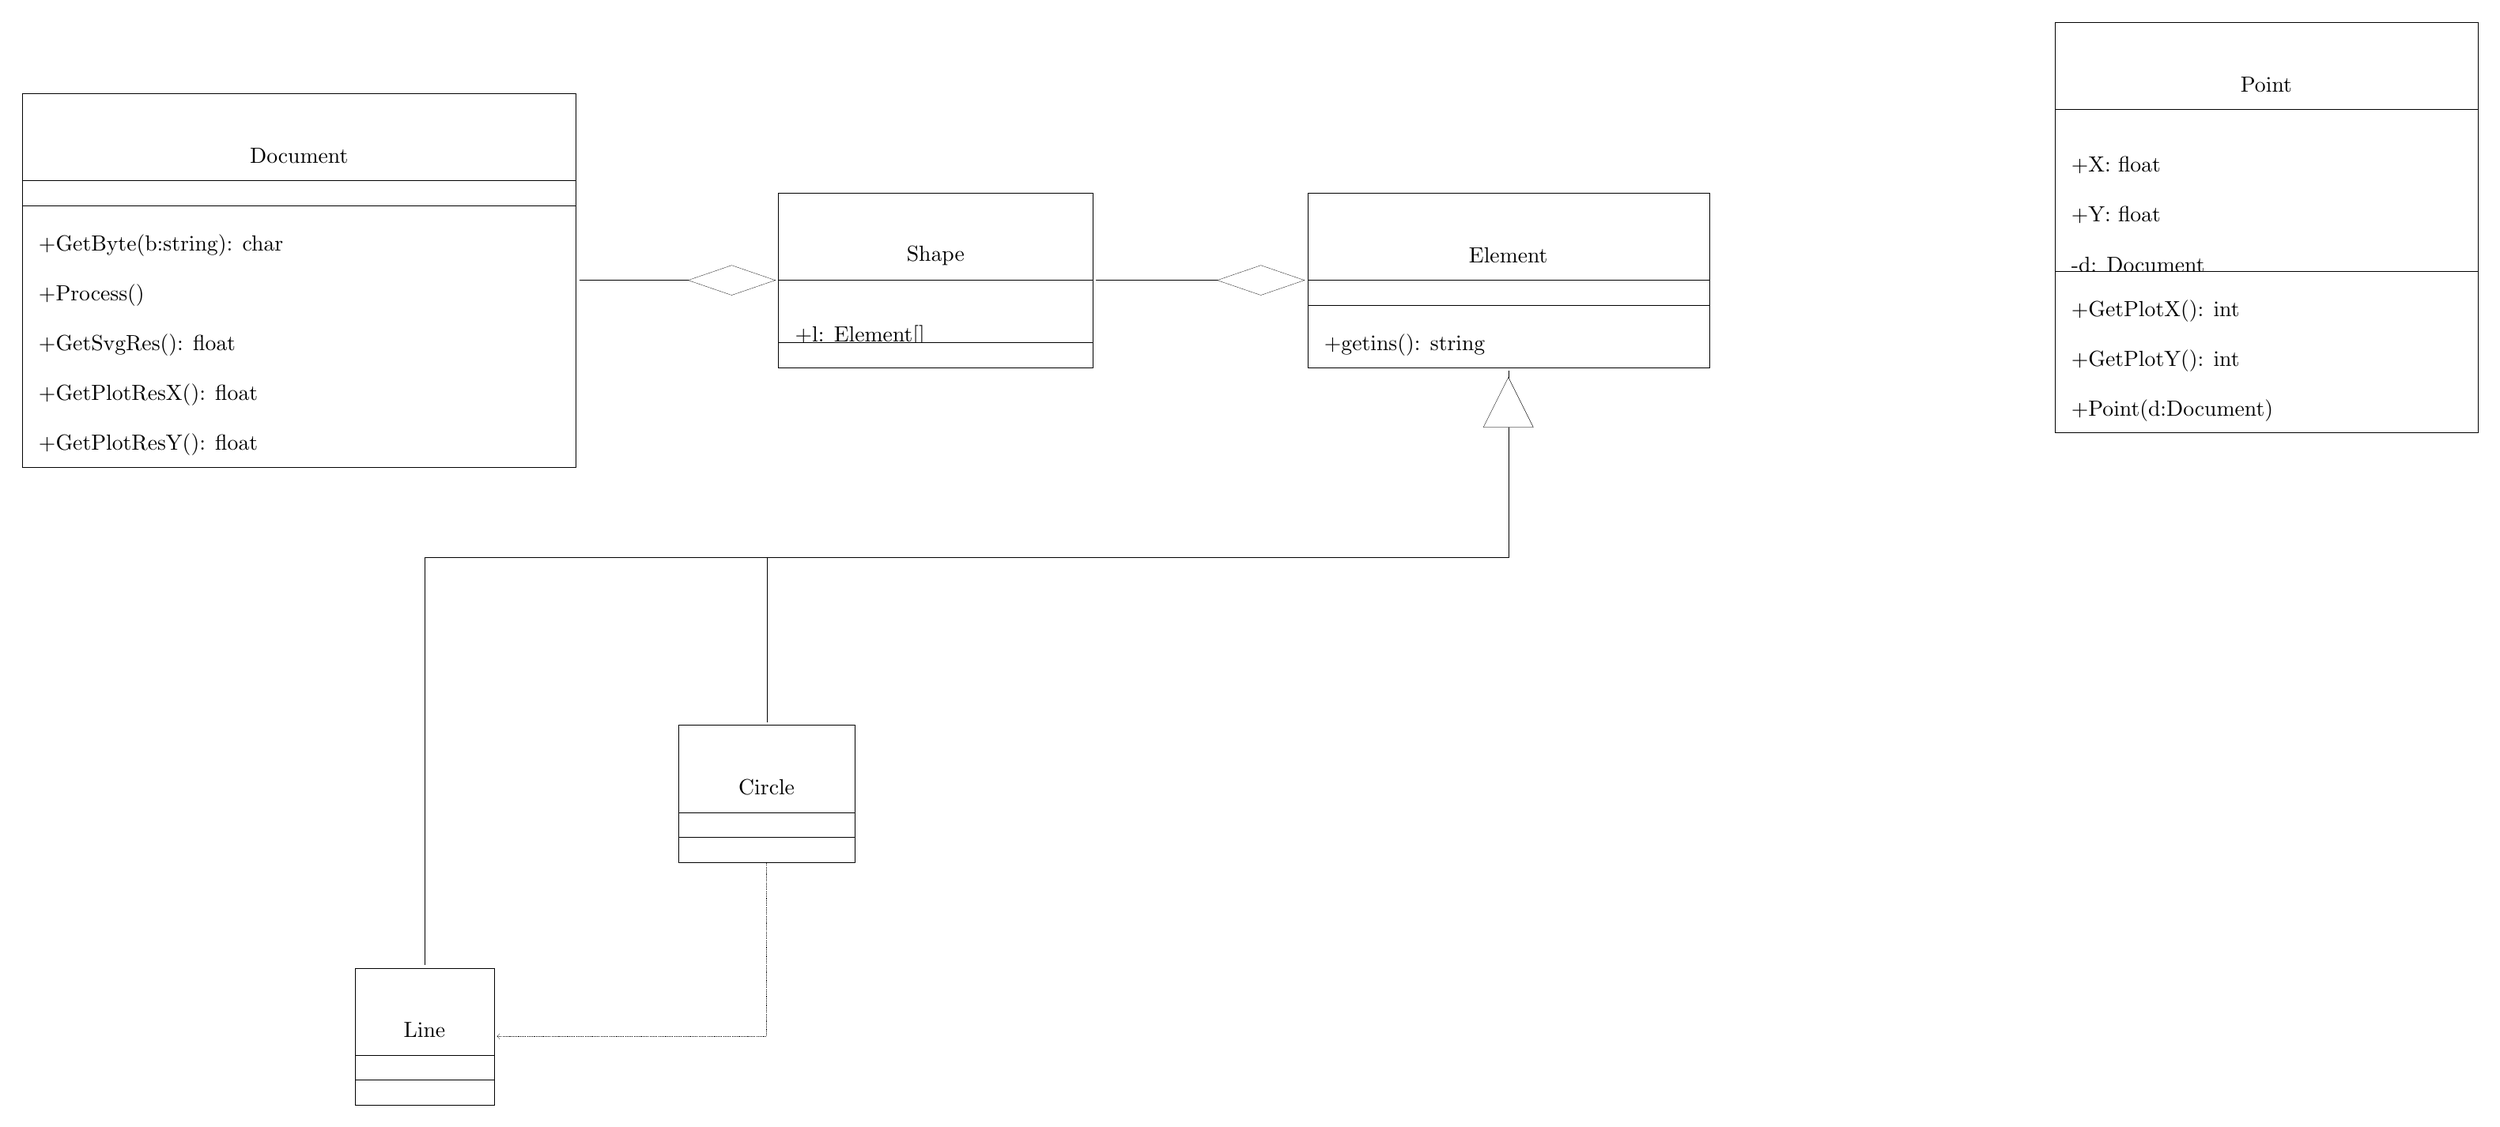
\begin{tikzpicture}
\pgftransformxscale{1.000000}
\pgftransformyscale{-1.000000}
\definecolor{dialinecolor}{rgb}{0.000000, 0.000000, 0.000000}
\pgfsetstrokecolor{dialinecolor}
\definecolor{dialinecolor}{rgb}{1.000000, 1.000000, 1.000000}
\pgfsetfillcolor{dialinecolor}
\pgfsetlinewidth{0.100000\du}
\pgfsetdash{}{0pt}
\definecolor{dialinecolor}{rgb}{1.000000, 1.000000, 1.000000}
\pgfsetfillcolor{dialinecolor}
\fill (0.750000\du,15.750000\du)--(0.750000\du,17.150000\du)--(9.650000\du,17.150000\du)--(9.650000\du,15.750000\du)--cycle;
\definecolor{dialinecolor}{rgb}{0.000000, 0.000000, 0.000000}
\pgfsetstrokecolor{dialinecolor}
\draw (0.750000\du,15.750000\du)--(0.750000\du,17.150000\du)--(9.650000\du,17.150000\du)--(9.650000\du,15.750000\du)--cycle;
% setfont left to latex
\definecolor{dialinecolor}{rgb}{0.000000, 0.000000, 0.000000}
\pgfsetstrokecolor{dialinecolor}
\node at (5.200000\du,16.750000\du){Document};
\definecolor{dialinecolor}{rgb}{1.000000, 1.000000, 1.000000}
\pgfsetfillcolor{dialinecolor}
\fill (0.750000\du,17.150000\du)--(0.750000\du,17.550000\du)--(9.650000\du,17.550000\du)--(9.650000\du,17.150000\du)--cycle;
\definecolor{dialinecolor}{rgb}{0.000000, 0.000000, 0.000000}
\pgfsetstrokecolor{dialinecolor}
\draw (0.750000\du,17.150000\du)--(0.750000\du,17.550000\du)--(9.650000\du,17.550000\du)--(9.650000\du,17.150000\du)--cycle;
\definecolor{dialinecolor}{rgb}{1.000000, 1.000000, 1.000000}
\pgfsetfillcolor{dialinecolor}
\fill (0.750000\du,17.550000\du)--(0.750000\du,21.750000\du)--(9.650000\du,21.750000\du)--(9.650000\du,17.550000\du)--cycle;
\definecolor{dialinecolor}{rgb}{0.000000, 0.000000, 0.000000}
\pgfsetstrokecolor{dialinecolor}
\draw (0.750000\du,17.550000\du)--(0.750000\du,21.750000\du)--(9.650000\du,21.750000\du)--(9.650000\du,17.550000\du)--cycle;
% setfont left to latex
\definecolor{dialinecolor}{rgb}{0.000000, 0.000000, 0.000000}
\pgfsetstrokecolor{dialinecolor}
\node[anchor=west] at (0.900000\du,18.192500\du){+GetByte(b:string): char};
% setfont left to latex
\definecolor{dialinecolor}{rgb}{0.000000, 0.000000, 0.000000}
\pgfsetstrokecolor{dialinecolor}
\node[anchor=west] at (0.900000\du,18.992500\du){+Process()};
% setfont left to latex
\definecolor{dialinecolor}{rgb}{0.000000, 0.000000, 0.000000}
\pgfsetstrokecolor{dialinecolor}
\node[anchor=west] at (0.900000\du,19.792500\du){+GetSvgRes(): float};
% setfont left to latex
\definecolor{dialinecolor}{rgb}{0.000000, 0.000000, 0.000000}
\pgfsetstrokecolor{dialinecolor}
\node[anchor=west] at (0.900000\du,20.592500\du){+GetPlotResX(): float};
% setfont left to latex
\definecolor{dialinecolor}{rgb}{0.000000, 0.000000, 0.000000}
\pgfsetstrokecolor{dialinecolor}
\node[anchor=west] at (0.900000\du,21.392500\du){+GetPlotResY(): float};
\pgfsetlinewidth{0.100000\du}
\pgfsetdash{}{0pt}
\definecolor{dialinecolor}{rgb}{1.000000, 1.000000, 1.000000}
\pgfsetfillcolor{dialinecolor}
\fill (12.900000\du,17.350000\du)--(12.900000\du,18.750000\du)--(17.950000\du,18.750000\du)--(17.950000\du,17.350000\du)--cycle;
\definecolor{dialinecolor}{rgb}{0.000000, 0.000000, 0.000000}
\pgfsetstrokecolor{dialinecolor}
\draw (12.900000\du,17.350000\du)--(12.900000\du,18.750000\du)--(17.950000\du,18.750000\du)--(17.950000\du,17.350000\du)--cycle;
% setfont left to latex
\definecolor{dialinecolor}{rgb}{0.000000, 0.000000, 0.000000}
\pgfsetstrokecolor{dialinecolor}
\node at (15.425000\du,18.350000\du){Shape};
\definecolor{dialinecolor}{rgb}{1.000000, 1.000000, 1.000000}
\pgfsetfillcolor{dialinecolor}
\fill (12.900000\du,18.750000\du)--(12.900000\du,19.750000\du)--(17.950000\du,19.750000\du)--(17.950000\du,18.750000\du)--cycle;
\definecolor{dialinecolor}{rgb}{0.000000, 0.000000, 0.000000}
\pgfsetstrokecolor{dialinecolor}
\draw (12.900000\du,18.750000\du)--(12.900000\du,19.750000\du)--(17.950000\du,19.750000\du)--(17.950000\du,18.750000\du)--cycle;
% setfont left to latex
\definecolor{dialinecolor}{rgb}{0.000000, 0.000000, 0.000000}
\pgfsetstrokecolor{dialinecolor}
\node[anchor=west] at (13.050000\du,19.650000\du){+l: Element\ensuremath{[}\ensuremath{]}};
\definecolor{dialinecolor}{rgb}{1.000000, 1.000000, 1.000000}
\pgfsetfillcolor{dialinecolor}
\fill (12.900000\du,19.750000\du)--(12.900000\du,20.150000\du)--(17.950000\du,20.150000\du)--(17.950000\du,19.750000\du)--cycle;
\definecolor{dialinecolor}{rgb}{0.000000, 0.000000, 0.000000}
\pgfsetstrokecolor{dialinecolor}
\draw (12.900000\du,19.750000\du)--(12.900000\du,20.150000\du)--(17.950000\du,20.150000\du)--(17.950000\du,19.750000\du)--cycle;
\pgfsetlinewidth{0.100000\du}
\pgfsetdash{}{0pt}
\definecolor{dialinecolor}{rgb}{1.000000, 1.000000, 1.000000}
\pgfsetfillcolor{dialinecolor}
\fill (21.400000\du,17.350000\du)--(21.400000\du,18.750000\du)--(27.850000\du,18.750000\du)--(27.850000\du,17.350000\du)--cycle;
\definecolor{dialinecolor}{rgb}{0.000000, 0.000000, 0.000000}
\pgfsetstrokecolor{dialinecolor}
\draw (21.400000\du,17.350000\du)--(21.400000\du,18.750000\du)--(27.850000\du,18.750000\du)--(27.850000\du,17.350000\du)--cycle;
% setfont left to latex
\definecolor{dialinecolor}{rgb}{0.000000, 0.000000, 0.000000}
\pgfsetstrokecolor{dialinecolor}
\node at (24.625000\du,18.350000\du){Element};
\definecolor{dialinecolor}{rgb}{1.000000, 1.000000, 1.000000}
\pgfsetfillcolor{dialinecolor}
\fill (21.400000\du,18.750000\du)--(21.400000\du,19.150000\du)--(27.850000\du,19.150000\du)--(27.850000\du,18.750000\du)--cycle;
\definecolor{dialinecolor}{rgb}{0.000000, 0.000000, 0.000000}
\pgfsetstrokecolor{dialinecolor}
\draw (21.400000\du,18.750000\du)--(21.400000\du,19.150000\du)--(27.850000\du,19.150000\du)--(27.850000\du,18.750000\du)--cycle;
\definecolor{dialinecolor}{rgb}{1.000000, 1.000000, 1.000000}
\pgfsetfillcolor{dialinecolor}
\fill (21.400000\du,19.150000\du)--(21.400000\du,20.150000\du)--(27.850000\du,20.150000\du)--(27.850000\du,19.150000\du)--cycle;
\definecolor{dialinecolor}{rgb}{0.000000, 0.000000, 0.000000}
\pgfsetstrokecolor{dialinecolor}
\draw (21.400000\du,19.150000\du)--(21.400000\du,20.150000\du)--(27.850000\du,20.150000\du)--(27.850000\du,19.150000\du)--cycle;
% setfont left to latex
\definecolor{dialinecolor}{rgb}{0.000000, 0.000000, 0.000000}
\pgfsetstrokecolor{dialinecolor}
\node[anchor=west] at (21.550000\du,19.792500\du){+getins(): string};
\pgfsetlinewidth{0.100000\du}
\pgfsetdash{}{0pt}
\definecolor{dialinecolor}{rgb}{1.000000, 1.000000, 1.000000}
\pgfsetfillcolor{dialinecolor}
\fill (6.100000\du,29.800000\du)--(6.100000\du,31.200000\du)--(8.330000\du,31.200000\du)--(8.330000\du,29.800000\du)--cycle;
\definecolor{dialinecolor}{rgb}{0.000000, 0.000000, 0.000000}
\pgfsetstrokecolor{dialinecolor}
\draw (6.100000\du,29.800000\du)--(6.100000\du,31.200000\du)--(8.330000\du,31.200000\du)--(8.330000\du,29.800000\du)--cycle;
% setfont left to latex
\definecolor{dialinecolor}{rgb}{0.000000, 0.000000, 0.000000}
\pgfsetstrokecolor{dialinecolor}
\node at (7.215000\du,30.800000\du){Line};
\definecolor{dialinecolor}{rgb}{1.000000, 1.000000, 1.000000}
\pgfsetfillcolor{dialinecolor}
\fill (6.100000\du,31.200000\du)--(6.100000\du,31.600000\du)--(8.330000\du,31.600000\du)--(8.330000\du,31.200000\du)--cycle;
\definecolor{dialinecolor}{rgb}{0.000000, 0.000000, 0.000000}
\pgfsetstrokecolor{dialinecolor}
\draw (6.100000\du,31.200000\du)--(6.100000\du,31.600000\du)--(8.330000\du,31.600000\du)--(8.330000\du,31.200000\du)--cycle;
\definecolor{dialinecolor}{rgb}{1.000000, 1.000000, 1.000000}
\pgfsetfillcolor{dialinecolor}
\fill (6.100000\du,31.600000\du)--(6.100000\du,32.000000\du)--(8.330000\du,32.000000\du)--(8.330000\du,31.600000\du)--cycle;
\definecolor{dialinecolor}{rgb}{0.000000, 0.000000, 0.000000}
\pgfsetstrokecolor{dialinecolor}
\draw (6.100000\du,31.600000\du)--(6.100000\du,32.000000\du)--(8.330000\du,32.000000\du)--(8.330000\du,31.600000\du)--cycle;
\pgfsetlinewidth{0.100000\du}
\pgfsetdash{}{0pt}
\definecolor{dialinecolor}{rgb}{1.000000, 1.000000, 1.000000}
\pgfsetfillcolor{dialinecolor}
\fill (11.300000\du,25.900000\du)--(11.300000\du,27.300000\du)--(14.122500\du,27.300000\du)--(14.122500\du,25.900000\du)--cycle;
\definecolor{dialinecolor}{rgb}{0.000000, 0.000000, 0.000000}
\pgfsetstrokecolor{dialinecolor}
\draw (11.300000\du,25.900000\du)--(11.300000\du,27.300000\du)--(14.122500\du,27.300000\du)--(14.122500\du,25.900000\du)--cycle;
% setfont left to latex
\definecolor{dialinecolor}{rgb}{0.000000, 0.000000, 0.000000}
\pgfsetstrokecolor{dialinecolor}
\node at (12.711250\du,26.900000\du){Circle};
\definecolor{dialinecolor}{rgb}{1.000000, 1.000000, 1.000000}
\pgfsetfillcolor{dialinecolor}
\fill (11.300000\du,27.300000\du)--(11.300000\du,27.700000\du)--(14.122500\du,27.700000\du)--(14.122500\du,27.300000\du)--cycle;
\definecolor{dialinecolor}{rgb}{0.000000, 0.000000, 0.000000}
\pgfsetstrokecolor{dialinecolor}
\draw (11.300000\du,27.300000\du)--(11.300000\du,27.700000\du)--(14.122500\du,27.700000\du)--(14.122500\du,27.300000\du)--cycle;
\definecolor{dialinecolor}{rgb}{1.000000, 1.000000, 1.000000}
\pgfsetfillcolor{dialinecolor}
\fill (11.300000\du,27.700000\du)--(11.300000\du,28.100000\du)--(14.122500\du,28.100000\du)--(14.122500\du,27.700000\du)--cycle;
\definecolor{dialinecolor}{rgb}{0.000000, 0.000000, 0.000000}
\pgfsetstrokecolor{dialinecolor}
\draw (11.300000\du,27.700000\du)--(11.300000\du,28.100000\du)--(14.122500\du,28.100000\du)--(14.122500\du,27.700000\du)--cycle;
\pgfsetlinewidth{0.100000\du}
\pgfsetdash{}{0pt}
\pgfsetmiterjoin
\pgfsetbuttcap
{
\definecolor{dialinecolor}{rgb}{0.000000, 0.000000, 0.000000}
\pgfsetfillcolor{dialinecolor}
% was here!!!
\definecolor{dialinecolor}{rgb}{0.000000, 0.000000, 0.000000}
\pgfsetstrokecolor{dialinecolor}
\draw (24.625000\du,20.199835\du)--(24.625000\du,23.200000\du)--(7.215000\du,23.200000\du)--(7.215000\du,29.753271\du);
}
\definecolor{dialinecolor}{rgb}{0.000000, 0.000000, 0.000000}
\pgfsetstrokecolor{dialinecolor}
\draw (24.625000\du,21.111639\du)--(24.625000\du,23.200000\du)--(7.215000\du,23.200000\du)--(7.215000\du,29.753271\du);
\pgfsetmiterjoin
\definecolor{dialinecolor}{rgb}{1.000000, 1.000000, 1.000000}
\pgfsetfillcolor{dialinecolor}
\fill (25.025000\du,21.111639\du)--(24.625000\du,20.311639\du)--(24.225000\du,21.111639\du)--cycle;
\pgfsetlinewidth{0.100000\du}
\pgfsetdash{}{0pt}
\pgfsetmiterjoin
\definecolor{dialinecolor}{rgb}{0.000000, 0.000000, 0.000000}
\pgfsetstrokecolor{dialinecolor}
\draw (25.025000\du,21.111639\du)--(24.625000\du,20.311639\du)--(24.225000\du,21.111639\du)--cycle;
% setfont left to latex
\pgfsetlinewidth{0.100000\du}
\pgfsetdash{}{0pt}
\pgfsetmiterjoin
\pgfsetbuttcap
{
\definecolor{dialinecolor}{rgb}{0.000000, 0.000000, 0.000000}
\pgfsetfillcolor{dialinecolor}
% was here!!!
\definecolor{dialinecolor}{rgb}{0.000000, 0.000000, 0.000000}
\pgfsetstrokecolor{dialinecolor}
\draw (24.625000\du,20.199835\du)--(24.625000\du,23.200000\du)--(12.711250\du,23.200000\du)--(12.711250\du,25.853320\du);
}
\definecolor{dialinecolor}{rgb}{0.000000, 0.000000, 0.000000}
\pgfsetstrokecolor{dialinecolor}
\draw (24.625000\du,21.111639\du)--(24.625000\du,23.200000\du)--(12.711250\du,23.200000\du)--(12.711250\du,25.853320\du);
\pgfsetmiterjoin
\definecolor{dialinecolor}{rgb}{1.000000, 1.000000, 1.000000}
\pgfsetfillcolor{dialinecolor}
\fill (25.025000\du,21.111639\du)--(24.625000\du,20.311639\du)--(24.225000\du,21.111639\du)--cycle;
\pgfsetlinewidth{0.100000\du}
\pgfsetdash{}{0pt}
\pgfsetmiterjoin
\definecolor{dialinecolor}{rgb}{0.000000, 0.000000, 0.000000}
\pgfsetstrokecolor{dialinecolor}
\draw (25.025000\du,21.111639\du)--(24.625000\du,20.311639\du)--(24.225000\du,21.111639\du)--cycle;
% setfont left to latex
\pgfsetlinewidth{0.100000\du}
\pgfsetdash{}{0pt}
\pgfsetmiterjoin
\pgfsetbuttcap
{
\definecolor{dialinecolor}{rgb}{0.000000, 0.000000, 0.000000}
\pgfsetfillcolor{dialinecolor}
% was here!!!
\definecolor{dialinecolor}{rgb}{0.000000, 0.000000, 0.000000}
\pgfsetstrokecolor{dialinecolor}
\draw (18.000314\du,18.750000\du)--(18.000314\du,18.750000\du)--(21.349600\du,18.750000\du)--(21.349600\du,18.750000\du);
}
\definecolor{dialinecolor}{rgb}{0.000000, 0.000000, 0.000000}
\pgfsetstrokecolor{dialinecolor}
\draw (18.000314\du,18.750000\du)--(18.000314\du,18.750000\du)--(20.091022\du,18.750000\du);
\pgfsetdash{}{0pt}
\pgfsetmiterjoin
\pgfsetbuttcap
\definecolor{dialinecolor}{rgb}{1.000000, 1.000000, 1.000000}
\pgfsetfillcolor{dialinecolor}
\fill (21.349600\du,18.750000\du)--(20.649600\du,18.990000\du)--(19.949600\du,18.750000\du)--(20.649600\du,18.510000\du)--cycle;
\pgfsetlinewidth{0.100000\du}
\pgfsetdash{}{0pt}
\pgfsetmiterjoin
\pgfsetbuttcap
\definecolor{dialinecolor}{rgb}{0.000000, 0.000000, 0.000000}
\pgfsetstrokecolor{dialinecolor}
\draw (21.349600\du,18.750000\du)--(20.649600\du,18.990000\du)--(19.949600\du,18.750000\du)--(20.649600\du,18.510000\du)--cycle;
% setfont left to latex
\definecolor{dialinecolor}{rgb}{0.000000, 0.000000, 0.000000}
\pgfsetstrokecolor{dialinecolor}
\node at (19.674957\du,18.750000\du){};
\pgfsetlinewidth{0.100000\du}
\pgfsetdash{{1.000000\du}{1.000000\du}}{0\du}
\pgfsetdash{{0.400000\du}{0.400000\du}}{0\du}
\pgfsetmiterjoin
\pgfsetbuttcap
{
\definecolor{dialinecolor}{rgb}{0.000000, 0.000000, 0.000000}
\pgfsetfillcolor{dialinecolor}
% was here!!!
\pgfsetarrowsend{to}
\definecolor{dialinecolor}{rgb}{0.000000, 0.000000, 0.000000}
\pgfsetstrokecolor{dialinecolor}
\draw (12.711250\du,28.100000\du)--(12.700000\du,28.100000\du)--(12.700000\du,30.900000\du)--(8.378688\du,30.900000\du);
}
% setfont left to latex
\pgfsetlinewidth{0.100000\du}
\pgfsetdash{}{0pt}
\pgfsetmiterjoin
\pgfsetbuttcap
{
\definecolor{dialinecolor}{rgb}{0.000000, 0.000000, 0.000000}
\pgfsetfillcolor{dialinecolor}
% was here!!!
\definecolor{dialinecolor}{rgb}{0.000000, 0.000000, 0.000000}
\pgfsetstrokecolor{dialinecolor}
\draw (9.700275\du,18.750000\du)--(9.700275\du,18.750000\du)--(12.849686\du,18.750000\du)--(12.849686\du,18.750000\du);
}
\definecolor{dialinecolor}{rgb}{0.000000, 0.000000, 0.000000}
\pgfsetstrokecolor{dialinecolor}
\draw (9.700275\du,18.750000\du)--(9.700275\du,18.750000\du)--(11.591107\du,18.750000\du);
\pgfsetdash{}{0pt}
\pgfsetmiterjoin
\pgfsetbuttcap
\definecolor{dialinecolor}{rgb}{1.000000, 1.000000, 1.000000}
\pgfsetfillcolor{dialinecolor}
\fill (12.849686\du,18.750000\du)--(12.149686\du,18.990000\du)--(11.449686\du,18.750000\du)--(12.149686\du,18.510000\du)--cycle;
\pgfsetlinewidth{0.100000\du}
\pgfsetdash{}{0pt}
\pgfsetmiterjoin
\pgfsetbuttcap
\definecolor{dialinecolor}{rgb}{0.000000, 0.000000, 0.000000}
\pgfsetstrokecolor{dialinecolor}
\draw (12.849686\du,18.750000\du)--(12.149686\du,18.990000\du)--(11.449686\du,18.750000\du)--(12.149686\du,18.510000\du)--cycle;
% setfont left to latex
\definecolor{dialinecolor}{rgb}{0.000000, 0.000000, 0.000000}
\pgfsetstrokecolor{dialinecolor}
\node[anchor=west] at (9.800275\du,18.750000\du){};
\pgfsetlinewidth{0.100000\du}
\pgfsetdash{}{0pt}
\definecolor{dialinecolor}{rgb}{1.000000, 1.000000, 1.000000}
\pgfsetfillcolor{dialinecolor}
\fill (33.400000\du,14.600000\du)--(33.400000\du,16.000000\du)--(40.200000\du,16.000000\du)--(40.200000\du,14.600000\du)--cycle;
\definecolor{dialinecolor}{rgb}{0.000000, 0.000000, 0.000000}
\pgfsetstrokecolor{dialinecolor}
\draw (33.400000\du,14.600000\du)--(33.400000\du,16.000000\du)--(40.200000\du,16.000000\du)--(40.200000\du,14.600000\du)--cycle;
% setfont left to latex
\definecolor{dialinecolor}{rgb}{0.000000, 0.000000, 0.000000}
\pgfsetstrokecolor{dialinecolor}
\node at (36.800000\du,15.600000\du){Point};
\definecolor{dialinecolor}{rgb}{1.000000, 1.000000, 1.000000}
\pgfsetfillcolor{dialinecolor}
\fill (33.400000\du,16.000000\du)--(33.400000\du,18.600000\du)--(40.200000\du,18.600000\du)--(40.200000\du,16.000000\du)--cycle;
\definecolor{dialinecolor}{rgb}{0.000000, 0.000000, 0.000000}
\pgfsetstrokecolor{dialinecolor}
\draw (33.400000\du,16.000000\du)--(33.400000\du,18.600000\du)--(40.200000\du,18.600000\du)--(40.200000\du,16.000000\du)--cycle;
% setfont left to latex
\definecolor{dialinecolor}{rgb}{0.000000, 0.000000, 0.000000}
\pgfsetstrokecolor{dialinecolor}
\node[anchor=west] at (33.550000\du,16.900000\du){+X: float};
% setfont left to latex
\definecolor{dialinecolor}{rgb}{0.000000, 0.000000, 0.000000}
\pgfsetstrokecolor{dialinecolor}
\node[anchor=west] at (33.550000\du,17.700000\du){+Y: float};
% setfont left to latex
\definecolor{dialinecolor}{rgb}{0.000000, 0.000000, 0.000000}
\pgfsetstrokecolor{dialinecolor}
\node[anchor=west] at (33.550000\du,18.500000\du){-d: Document};
\definecolor{dialinecolor}{rgb}{1.000000, 1.000000, 1.000000}
\pgfsetfillcolor{dialinecolor}
\fill (33.400000\du,18.600000\du)--(33.400000\du,21.200000\du)--(40.200000\du,21.200000\du)--(40.200000\du,18.600000\du)--cycle;
\definecolor{dialinecolor}{rgb}{0.000000, 0.000000, 0.000000}
\pgfsetstrokecolor{dialinecolor}
\draw (33.400000\du,18.600000\du)--(33.400000\du,21.200000\du)--(40.200000\du,21.200000\du)--(40.200000\du,18.600000\du)--cycle;
% setfont left to latex
\definecolor{dialinecolor}{rgb}{0.000000, 0.000000, 0.000000}
\pgfsetstrokecolor{dialinecolor}
\node[anchor=west] at (33.550000\du,19.242500\du){+GetPlotX(): int};
% setfont left to latex
\definecolor{dialinecolor}{rgb}{0.000000, 0.000000, 0.000000}
\pgfsetstrokecolor{dialinecolor}
\node[anchor=west] at (33.550000\du,20.042500\du){+GetPlotY(): int};
% setfont left to latex
\definecolor{dialinecolor}{rgb}{0.000000, 0.000000, 0.000000}
\pgfsetstrokecolor{dialinecolor}
\node[anchor=west] at (33.550000\du,20.842500\du){+Point(d:Document)};
\end{tikzpicture}

  \caption{Oversigt over objekter}
  \label{fig:obj-oversigt}
\end{figure}


\end{document}

%%% Local Variables:
%%% mode: latex
%%% End: